% questions.tex —— 2005 年·普通高等学校招生考试·江西卷·理科 · 题目内容片段（无答案）
% 由 tools/generate_projects.py 依来源总账自 2005/2005_数学真题_江西理科_试题.md 生成，勿手改（改源 MD 后重跑）

\gkpart{一、选择题：本大题共 12 小题，每小题 5 分，共 60 分．在每小题给出的四个选项中，只有一项是符合题目要求的．}

\begin{question}
\gkti{1}设集合 $I = \{x \mid |x| < 3, x \in \mathbf{Z}\}, A = \{1, 2\}, B = \{-2, -1, 2\}$，则 $A \cup (\complement_I B) =$\mbox{（　　）}

\begin{gkopts}(4)
\task A．$\{1\}$
\task B．$\{1, 2\}$
\task C．$\{2\}$
\task D．$\{0, 1, 2\}$
\end{gkopts}

\end{question}
\begin{question}
\gkti{2}设复数：$z_1 = 1 + \mathrm{i}, z_2 = x + 2\mathrm{i}\ (x \in \mathbf{R})$，若 $z_1 z_2$ 为实数，则 $x =$\mbox{（　　）}

\begin{gkopts}(4)
\task A．$-2$
\task B．$-1$
\task C．$1$
\task D．$2$
\end{gkopts}

\end{question}
\begin{question}
\gkti{3}“$a = b$”是“直线 $y = x + 2$ 与圆 $(x - a)^2 + (y + b)^2 = 2$ 相切”的\mbox{（　　）}

\begin{gkopts}(2)
\task A．充分不必要条件
\task B．必要不充分条件
\task C．充分必要条件
\task D．既不充分又不必要条件
\end{gkopts}

\end{question}
\begin{question}
\gkti{4}$(\sqrt{x} + \sqrt[3]{x})^{12}$ 的展开式中，含 $x$ 的正整数次幂的项共有\mbox{（　　）}

\begin{gkopts}(4)
\task A．4 项
\task B．3 项
\task C．2 项
\task D．1 项
\end{gkopts}

\end{question}
\begin{question}
\gkti{5}设函数 $f(x) = \sin 3x + |\sin 3x|$，则 $f(x)$ 为\mbox{（　　）}

\begin{gkopts}(2)
\task A．周期函数，最小正周期为 $\dfrac{\pi}{3}$
\task B．周期函数，最小正周期为 $\dfrac{2\pi}{3}$
\task C．周期函数，最小正周期为 $2\pi$
\task D．非周期函数
\end{gkopts}

\end{question}
\begin{question}
\gkti{6}已知向量 $\vec{a} = (1, 2), \vec{b} = (-2, -4), |\vec{c}| = \sqrt{5}$，若 $(\vec{a} + \vec{b}) \cdot \vec{c} = \dfrac{5}{2}$，则 $\vec{a}$ 与 $\vec{c}$ 的夹角为\mbox{（　　）}

\begin{gkopts}(4)
\task A．$30^\circ$
\task B．$60^\circ$
\task C．$120^\circ$
\task D．$150^\circ$
\end{gkopts}

\Needspace{0.4\textheight}
\end{question}
\begin{question}
\gkti{7}已知函数 $y = xf'(x)$ 的图象如图所示（其中 $f'(x)$ 是函数 $f(x)$ 的导函数），下面四个图象中，$y = f(x)$ 的图象大致是\mbox{（　　）}
\nopagebreak[4]
\begin{center}% 2005 年江西卷理科第 7 题题干图：y = x f'(x) 图象
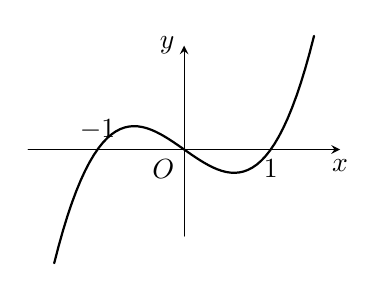
\begin{tikzpicture}[>=stealth,scale=1.1,line cap=round]
  \draw[->] (-1.8,0) -- (1.8,0) node[below] {$x$};
  \draw[->] (0,-1.0) -- (0,1.2) node[left] {$y$};
  \node[below left] at (0,0) {$O$};
  \draw[thick,domain=-1.5:1.5,samples=60] plot (\x,{\x*(\x*\x - 1)*0.7});
  \node[above] at (-1,0) {$-1$};
  \node[below] at (1,0) {$1$};
\end{tikzpicture}
\end{center}
\nopagebreak[4]
\nopagebreak[4]
\begin{center}% 2005 年江西卷理科第 7 题选项图：y = f(x) 4 个选项 (A)~(D)
\begin{tikzpicture}[>=stealth,scale=0.75,line cap=round]
  % (A)
  \begin{scope}
    \draw[->] (-2.6,0) -- (2.6,0) node[below] {$x$};
    \draw[->] (0,-0.8) -- (0,3.3) node[left] {$y$};
    \node[below right] at (0,0) {$O$};
    \foreach \x in {-2,-1,1,2} \draw (\x,0.05) -- (\x,-0.05);
    \node[below] at (-2,0) {$-2$};
    \node[below] at (-1,0) {$-1$};
    \node[below] at (1,0) {$1$};
    \node[below] at (2,0) {$2$};
    \foreach \y in {1,2} \draw (0.05,\y) -- (-0.05,\y) node[left] {$\y$};
    \draw[thick,domain=-2.4:2.3,samples=50] plot (\x,{-0.45*(\x+1.2)*(\x-1.8)*(\x-1.8) + 1.2});
    \node at (-1.8,-1.2) {(A)};
  \end{scope}

  % (B)
  \begin{scope}[xshift=6.5cm]
    \draw[->] (-2.6,0) -- (2.6,0) node[below] {$x$};
    \draw[->] (0,-0.8) -- (0,3.3) node[left] {$y$};
    \node[above left] at (0,0) {$O$};
    \foreach \x in {-2,-1,1,2} \draw (\x,0.05) -- (\x,-0.05);
    \node[below] at (-2,0) {$-2$};
    \node[below] at (-1,0) {$-1$};
    \node[below] at (1,0) {$1$};
    \node[below] at (2,0) {$2$};
    \foreach \y in {1,2} \draw (0.05,\y) -- (-0.05,\y) node[left] {$\y$};
    \draw[thick,domain=-1.3:1.8,samples=50] plot (\x,{-0.8*(\x+0.6)*(\x-1.2)*(\x-1.2) + 0.6});
    \node at (-1.8,-1.2) {(B)};
  \end{scope}

  % (C) 正确选项：x=-1 极大值，x=1 极小值
  \begin{scope}[yshift=-5.5cm]
    \draw[->] (-2.6,0) -- (2.6,0) node[below] {$x$};
    \draw[->] (0,-0.8) -- (0,3.3) node[left] {$y$};
    \node[below left] at (0,0) {$O$};
    \foreach \x in {-2,-1,1,2} \draw (\x,0.05) -- (\x,-0.05);
    \node[above left] at (-2,0) {$-2$};
    \node[below] at (-1,0) {$-1$};
    \node[below] at (1,0) {$1$};
    \node[below] at (2,0) {$2$};
    \foreach \y in {1,2} \draw (0.05,\y) -- (-0.05,\y) node[left] {$\y$};
    \draw[thick,domain=-2.3:2.2,samples=50] plot (\x,{0.6*(\x-1)*(\x-1)*(\x+2)});
    \node at (-1.8,-1.2) {(C)};
  \end{scope}

  % (D)
  \begin{scope}[xshift=6.5cm,yshift=-5.5cm]
    \draw[->] (-2.6,0) -- (2.6,0) node[below] {$x$};
    \draw[->] (0,-0.8) -- (0,3.3) node[left] {$y$};
    \node[below right] at (0,0) {$O$};
    \foreach \x in {-2,-1,1,2} \draw (\x,0.05) -- (\x,-0.05);
    \node[below] at (-2,0) {$-2$};
    \node[below] at (-1,0) {$-1$};
    \node[below] at (1,0) {$1$};
    \node[below] at (2,0) {$2$};
    \foreach \y in {1,2} \draw (0.05,\y) -- (-0.05,\y) node[left] {$\y$};
    \draw[thick,domain=-2.2:2.4,samples=50] plot (\x,{0.35*(\x-2)*(\x-2)*(\x+1.8)});
    \node at (-1.8,-1.2) {(D)};
  \end{scope}
\end{tikzpicture}
\end{center}
\nopagebreak[4]
\end{question}
\begin{question}
\gkti{8}若 $\lim_{x \to 1} \dfrac{f(x-1)}{x-1} = 1$，则 $\lim_{x \to 1} \dfrac{x-1}{f(2-2x)} =$\mbox{（　　）}

\begin{gkopts}(4)
\task A．$-1$
\task B．$1$
\task C．$-\dfrac{1}{2}$
\task D．$\dfrac{1}{2}$
\end{gkopts}

\end{question}
\begin{question}
\gkti{9}矩形 $ABCD$ 中，$AB = 4, BC = 3$，沿 $AC$ 将矩形 $ABCD$ 折成一个直二面角 $B - AC - D$，则四面体 $ABCD$ 的外接球的体积为\mbox{（　　）}

\begin{gkopts}(2)
\task A．$\dfrac{125}{12}\pi$
\task B．$\dfrac{125}{9}\pi$
\task C．$\dfrac{125}{6}\pi$
\task D．$\dfrac{125}{3}\pi$
\end{gkopts}

\end{question}
\begin{question}
\gkti{10}已知实数 $a, b$ 满足等式 $\left(\dfrac{1}{2}\right)^a = \left(\dfrac{1}{3}\right)^b$，下列五个关系式：
① $0 < b < a$；② $a < b < 0$；③ $0 < a < b$；④ $b < a < 0$；⑤ $a = b$．
其中不可能成立的关系式有\mbox{（　　）}

\begin{gkopts}(4)
\task A．1 个
\task B．2 个
\task C．3 个
\task D．4 个
\end{gkopts}

\end{question}
\begin{question}
\gkti{11}在 $\triangle OAB$ 中，$O$ 为坐标原点，$A(1, \cos\theta), B(\sin\theta, 1), \theta \in \left(0, \dfrac{\pi}{2}\right]$，则 $\triangle OAB$ 的面积达到最大值时，$\theta =$\mbox{（　　）}

\begin{gkopts}(4)
\task A．$\dfrac{\pi}{6}$
\task B．$\dfrac{\pi}{4}$
\task C．$\dfrac{\pi}{3}$
\task D．$\dfrac{\pi}{2}$
\end{gkopts}

\end{question}
\begin{question}
\gkti{12}将 $1, 2, \dots, 9$ 这 9 个数平均分成三组，则每组的三个数都成等差数列的概率为\mbox{（　　）}

\begin{gkopts}(4)
\task A．$\dfrac{1}{56}$
\task B．$\dfrac{1}{70}$
\task C．$\dfrac{1}{336}$
\task D．$\dfrac{1}{420}$
\end{gkopts}

\end{question}
\gkpart{二、填空题：本大题共 4 小题，每小题 4 分，共 16 分．把答案填在题中横线上．}

\begin{question}
\gkti{13}若函数 $f(x) = \log_a(x + \sqrt{x^2 + 2a^2})$ 是奇函数，则 $a = \underline{\hspace{2em}}$．

\end{question}
\begin{question}
\gkti{14}设实数 $x, y$ 满足 $\begin{cases} x - y - 2 \leqslant 0, \\ x + 2y - 4 > 0, \\ 2y - 3 \leqslant 0, \end{cases}$ 则 $\dfrac{y}{x}$ 的最大值是 $\underline{\hspace{2em}}$．

\Needspace{0.4\textheight}
\end{question}
\begin{question}
\gkti{15}如图，在直三棱柱 $ABC - A_1B_1C_1$ 中，$AB = BC = \sqrt{2}, BB_1 = 2, \angle ABC = 90^\circ$，$E, F$ 分别为 $AA_1, C_1B_1$ 的中点，沿棱柱的表面从 $E$ 到 $F$ 两点的最短路径的长度为 $\underline{\hspace{2em}}$．
\nopagebreak[4]
\begin{center}% 2005 年江西卷理科第 15 题：直三棱柱表面最短路径
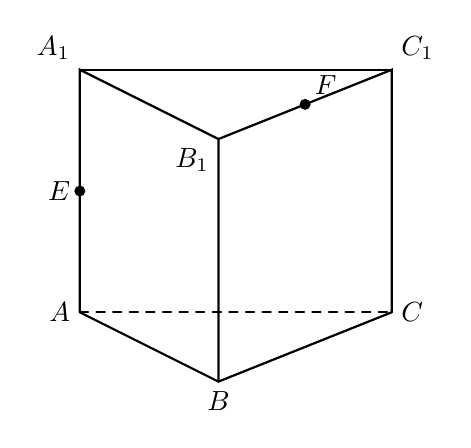
\begin{tikzpicture}[>=stealth,scale=1.1,line cap=round]
  \coordinate (A) at (0, 0.8);
  \coordinate (B) at (1.6, 0);
  \coordinate (C) at (3.6, 0.8);
  \coordinate (A1) at (0, 3.6);
  \coordinate (B1) at (1.6, 2.8);
  \coordinate (C1) at (3.6, 3.6);
  \coordinate (E) at (0, 2.2);
  \coordinate (F) at (2.6, 3.2);

  % 棱线
  \draw[thick] (A) -- (B) -- (C);
  \draw[dashed,thick] (A) -- (C);
  \draw[thick] (A) -- (A1) -- (B1) -- (B);
  \draw[thick] (B1) -- (C1) -- (C);
  \draw[thick] (A1) -- (C1);

  % 点 E, F
  \fill (E) circle (1.8pt) node[left] {$E$};
  \fill (F) circle (1.8pt) node[above right] {$F$};

  % 顶点标注
  \node[left] at (A) {$A$};
  \node[below] at (B) {$B$};
  \node[right] at (C) {$C$};
  \node[above left] at (A1) {$A_1$};
  \node[below left] at (B1) {$B_1$};
  \node[above right] at (C1) {$C_1$};
\end{tikzpicture}
\end{center}
\nopagebreak[4]
\end{question}
\begin{question}
\gkti{16}以下四个关于圆锥曲线的命题中：
① 设 $A, B$ 为两个定点，$k$ 为非零常数，$||\vec{PA}| - |\vec{PB}|| = k$，则动点 $P$ 的轨迹为双曲线；
② 设定圆 $C$ 上一定点 $A$ 作圆的动点弦 $AB$，$O$ 为坐标原点，若 $\vec{OP} = \dfrac{1}{2}(\vec{OA} + \vec{OB})$，则动点 $P$ 的轨迹为椭圆；
③ 方程 $2x^2 - 5x + 2 = 0$ 的两根可分别作为椭圆和双曲线的离心率；
④ 双曲线 $\dfrac{x^2}{25} - \dfrac{y^2}{9} = 1$ 与椭圆 $\dfrac{x^2}{35} + y^2 = 1$ 有相同的焦点．
其中真命题的序号为 $\underline{\hspace{2em}}$．（写出所有真命题的序号）

\end{question}
\gkpart{三、解答题：本大题共 6 小题，共 74 分．解答应写出文字说明、证明过程或演算步骤．}

\begin{question}
\gkti{17}已知函数 $f(x) = \dfrac{x^2}{ax + b}$（$a, b$ 为常数），且方程 $f(x) - x + 12 = 0$ 有两个实根为 $x_1 = 3, x_2 = 4$．
(1) 求函数 $f(x)$ 的解析式；
(2) 设 $k > 1$，解关于 $x$ 的不等式：$f(x) < \dfrac{(k+1)x - k}{2-x}$．

\end{question}
\begin{question}
\gkti{18}已知向量 $\vec{a} = \left(2\cos\dfrac{x}{2}, \tan\left(\dfrac{x}{2} + \dfrac{\pi}{4}\right)\right)$，$\vec{b} = \left(\sqrt{2}\sin\left(\dfrac{x}{2} + \dfrac{\pi}{4}\right), \tan\left(\dfrac{x}{2} - \dfrac{\pi}{4}\right)\right)$，令 $f(x) = \vec{a} \cdot \vec{b}$．是否存在实数 $x \in [0, \pi]$，使 $f(x) + f'(x) = 0$（其中 $f'(x)$ 是 $f(x)$ 的导函数）？若存在，则求出 $x$ 的值；若不存在，则证明之．

\end{question}
\begin{question}
\gkti{19}A、B 两位同学各有五张卡片，现以投掷均匀硬币的形式进行游戏，当出现正面朝上时 A 赢得 B 一张卡片，否则 B 赢得 A 一张卡片．规定掷硬币的次数达 9 次时，或在此前某人已赢得所有卡片时游戏终止．设 $\xi$ 表示游戏终止时掷硬币的次数．
(1) 求 $\xi$ 的取值范围；
(2) 求 $\xi$ 的数学期望 $\mathbf{E}\xi$．

\Needspace{0.4\textheight}
\end{question}
\begin{question}
\gkti{20}如图，在长方体 $ABCD - A_1B_1C_1D_1$ 中，$AD = AA_1 = 1, AB = 2$，点 $E$ 在棱 $AB$ 上移动．
(1) 证明：$D_1E \perp A_1D$；
(2) 当 $E$ 为 $AB$ 的中点时，求点 $E$ 到面 $ACD_1$ 的距离；
(3) $AE$ 等于何值时，二面角 $D_1 - EC - D$ 的大小为 $\dfrac{\pi}{4}$．
\nopagebreak[4]
\begin{center}% 2005 年江西卷理科第 20 题：长方体与截面 D1EC
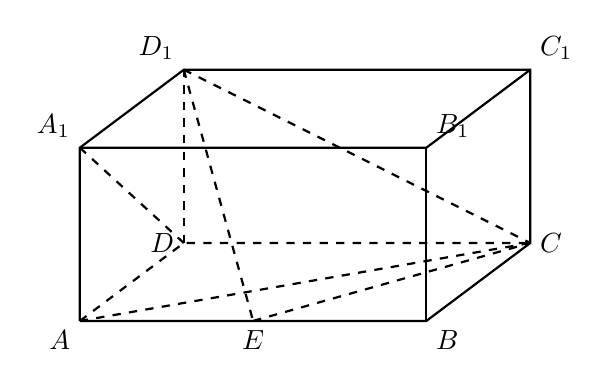
\begin{tikzpicture}[scale=1.1,>=stealth]
  % 顶点坐标
  \coordinate (A) at (0, 0);
  \coordinate (B) at (4.0, 0);
  \coordinate (D) at (1.2, 0.9);
  \coordinate (C) at (5.2, 0.9);

  \coordinate (A1) at (0, 2.0);
  \coordinate (B1) at (4.0, 2.0);
  \coordinate (D1) at (1.2, 2.9);
  \coordinate (C1) at (5.2, 2.9);

  % 点 E 位于 AB 上
  \coordinate (E) at (2.0, 0);

  % 长方体可见棱
  \draw[thick] (A) -- (B) -- (C) -- (C1) -- (D1) -- (A1) -- (A);
  \draw[thick] (A1) -- (B1) -- (C1);
  \draw[thick] (B) -- (B1);

  % 长方体内部不可见棱 (虚线)
  \draw[dashed, thick] (A) -- (D) -- (C);
  \draw[dashed, thick] (D) -- (D1);

  % 辅助线与线段 (虚线)
  \draw[dashed, thick] (D1) -- (E);
  \draw[dashed, thick] (E) -- (C);
  \draw[dashed, thick] (D1) -- (C);
  \draw[dashed, thick] (A) -- (C);
  \draw[dashed, thick] (A1) -- (D);

  % 顶点标签
  \node[below left] at (A) {$A$};
  \node[below right] at (B) {$B$};
  \node[right] at (C) {$C$};
  \node[left] at (D) {$D$};
  \node[above left] at (A1) {$A_1$};
  \node[above right] at (B1) {$B_1$};
  \node[above right] at (C1) {$C_1$};
  \node[above left] at (D1) {$D_1$};
  \node[below] at (E) {$E$};
\end{tikzpicture}
\end{center}
\nopagebreak[4]
\end{question}
\begin{question}
\gkti{21}已知数列 $\{a_n\}$ 的各项都是正数，且满足：$a_0 = 1$，$a_{n+1} = \dfrac{1}{2}a_n(4 - a_n)\ (n \in \mathbf{N})$．
(1) 证明：$a_n < a_{n+1} < 2\ (n \in \mathbf{N})$；
(2) 求数列 $\{a_n\}$ 的通项公式 $a_n$．

\Needspace{0.4\textheight}
\end{question}
\begin{question}
\gkti{22}如图，设抛物线 $C: y = x^2$ 的焦点为 $F$，动点 $P$ 在直线 $l: x - y - 2 = 0$ 上运动，过 $P$ 作抛物线 $C$ 的两条切线 $PA, PB$，且与抛物线 $C$ 分别相切于 $A, B$ 两点．
(1) 求 $\triangle APB$ 的重心 $G$ 的轨迹方程；
(2) 证明 $\angle PFA = \angle PFB$．
\nopagebreak[4]
\begin{center}% 2005 年江西卷理科第 22 题：抛物线切线与焦点角
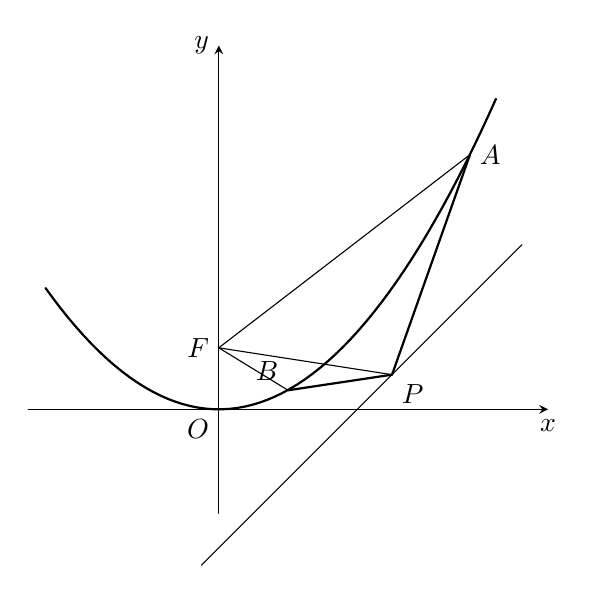
\begin{tikzpicture}[>=stealth,scale=1.1,line cap=round]
  % 坐标轴
  \draw[->] (-2.2,0) -- (3.8,0) node[below] {$x$};
  \draw[->] (0,-1.2) -- (0,4.2) node[left] {$y$};
  \node[below left] at (0,0) {$O$};

  % 抛物线 y = 0.35 x^2
  \draw[thick,domain=-2.0:3.2,samples=60] plot (\x,{0.35*\x*\x});

  % 关键点坐标
  \coordinate (F) at (0, 0.71);
  \coordinate (P) at (2.0, 0.4);
  \coordinate (A) at (2.9, 2.94);
  \coordinate (B) at (0.8, 0.22);

  % 直线 l: y = x - 1.6 通过 P(2.0, 0.4)
  \draw[domain=-0.2:3.5,samples=2] plot (\x,{\x - 1.6});

  % 切线 PA, PB
  \draw[thick] (P) -- (A);
  \draw[thick] (P) -- (B);

  % 焦点连线 FA, FB, FP
  \draw (F) -- (A);
  \draw (F) -- (B);
  \draw (F) -- (P);

  % 点标注
  \node[left] at (F) {$F$};
  \node[right] at (A) {$A$};
  \node[below right] at (P) {$P$};
  \node[above left] at (B) {$B$};
\end{tikzpicture}
\end{center}
\nopagebreak[4]

\end{question}